\documentclass[a4paper,11pt]{article}

\usepackage[spanish]{babel}
\usepackage[utf8]{inputenc}

\usepackage{amsmath}
\usepackage{siunitx}

\usepackage{graphicx}
\usepackage{float}
\usepackage[font=small,labelfont=bf]{caption}
\usepackage[colorlinks=true]{hyperref}

\usepackage{booktabs}
\usepackage{multirow}

\title{Caracterización de componentes electrónicos utilizando una placa de audio}
\date{\today}
\author{Micaela Toscani, Axel Lacapmesure y Guillermo Brinatti}

\begin{document}
\maketitle



\section{Introducción}

\section{Desarrollo de la aplicación de adquisición}
\label{sec:software}

	El control de la placa de adquisición fue llevado a cabo a partir de programar una biblioteca propia en lenguaje Python \cite{repo}. La misma incluyó funciones orientadas al usuario final destinadas a utilizar el dispositivo para la adquisición de datos y la generación de trenes de pulsos configurables, tanto en los modos de disparo único como de ejecución continua. Para ello empleamos la biblioteca \emph{\href{https://nidaqmx-python.readthedocs.io}{nidaqmx}} propia del fabricante de la placa de adquisición \cite{nidaqmx}, y que provee una API para la configuración del dispositivo y para su comunicación a través de los controladores del mismo.
	
	Las funciones de usuario final se encargaron de la configuración de los canales de entrada analógicos y salidas de contadores, de la adquisición de una muestra finita de largo arbitrario, y de la adquisición continua de datos en simultáneo con la generación de pulsos de anchos variables. En la figura \ref{fig:flujo_software} se muestra un diagrama de flujo de una ejecución típica para la adquisición y generación de pulsos en modo continuo. Asimismo la biblioteca incluyó los elementos necesarios para la implementación del lazo de control que se discutirá en la sección \ref{sec:control_temperatura}, a saber, las estructuras que manejan la entrada de datos de sensado, que calculan la señal de error y que generan la señal de hacia el actuador.
	
	El la adquisición de lectura y escritura se basa en un bucle que en cada iteración adquiere una ventana de datos con un número fijo de muestras, las procesa y por último escribe la configuración de los pulsos de salida, esto es, su frecuencia de repetición y su ancho. Para el funcionamiento de este esquema se asume que el tiempo de ejecución de las instrucciones dentro de cada iteración es menor al tiempo que demora la adquisición de las muestras, de manera que no se produzcan sobrecargas en el \emph{buffer} de la placa de adquisición. Bajo el modo de disparo único, las sucesivas ventanas temporales se concatenan en una variable de salida preinicializada, y el bucle finaliza cuando el número de muestras adquiridas alcanza el número total configurado. Bajo el modo de ejecucuón continua, las ventanas temporales se sobreescriben, y el bucle finaliza cuando el usuario interrumpe manualmente la ejecución del programa con el comando de teclado. En ambos casos, la finalización del bucle desencadena la etapa de cierre de comunicaciones y, eventualmente, el gráfico y guardado de los datos.
	
	\begin{figure}[!h] 
        \centering
        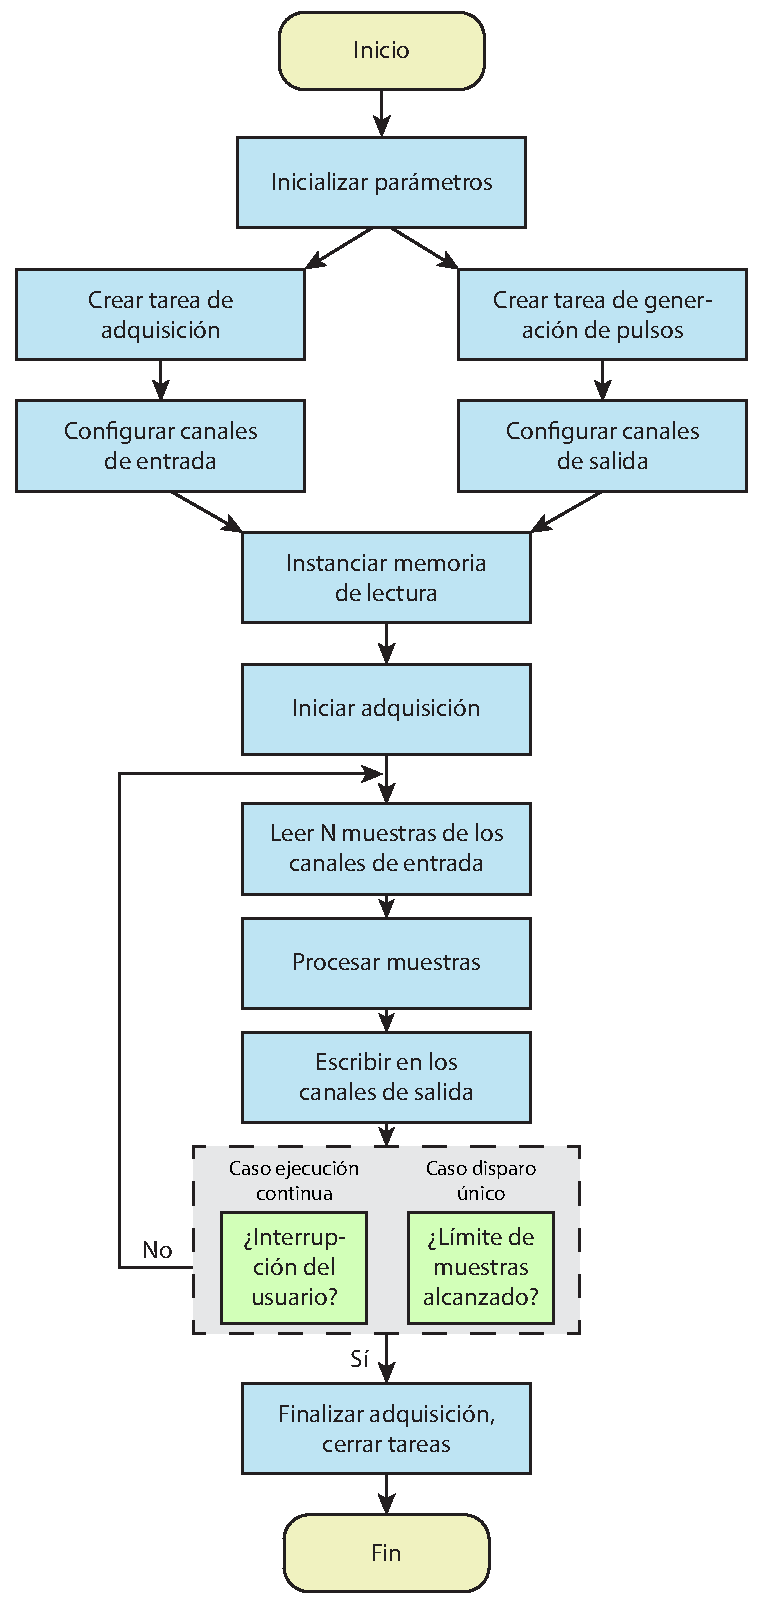
\includegraphics[height=.95\textheight]{flujo_software.pdf}
        \caption{Diagrama de flujo para la aplicación de adquisición y generación de pulsos en modo de disparo único y ejecución continua.}
        \label{fig:flujo_software}
 
    \end{figure}
	

\section{Caracterización de la placa de adquisición}

Se realizó una caracterización de la placa de adquisición en la que se propuso investigar los efectos de \textit{aliasing}, los tiempos asociados al multiplexado y el efecto del \textit{settling time} de la placa en las mediciones analógicas. 

En primer lugar, para observar el efecto que produce submuestrear una señal, se alimento una entrada analógica de la placa DAQ con una señal sinusoidal de frecuencia controlada producida por un generador de funciones. Se fijó la frecuencia de muestreo de la placa en $f_s$ = 10 kHz y se barrió la frecuencia de la señal de entrada $f_r$ entre valores mucho menores y mucho mayores a dicha frecuencia. El tiempo de integración se eligió grande, de manera de minimizar la introducción de frecuencias espúreas en la señal dadas por el tamaño de la ventana temporal. Luego, usando un algoritmo de tranformada rápida de Fourier (FFT), se obtuvo para cada frecuencia de entrada su frecuencia medida $f_m$, a partir del valor máximo del módulo de la FFT. En la figura \ref{fig:aliasing} se muestran los resultados de este experimento. Para frecuencias menores a la frecuencia de Nyquist ($f_r/f_s = 0.5$) se observa como la frecuencia medida se corresponde con la de la señal de entrada. A partir de este punto, se puede ver como el algoritmo devuelve de manera consistente valores menores a la frecuencia de Nyquist mostrando el fenómeno de aliasing. En particular, el punto donde $f_r = f_s$ devuelve un valor de frecuencia nulo, que se corresponde con estar muestreando la señal en el mismo punto del período cada vez.

\begin{figure}[h!]
\centering
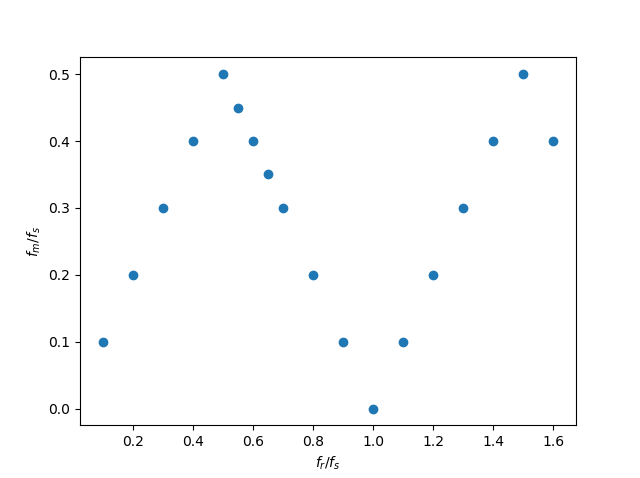
\includegraphics[width=\columnwidth]{figs/alliasing.png}
\label{fig:aliasing}
\caption{Frecuencia medida en función de la frecuencia real comparadas con la tasa de muestreo.}
\end{figure}

Para entender la forma en que la placa multiplexa las señales, se diseño un experimento en el que se busca medir cual es la relación entre los tiempos en los que se efectúa la adquisición para cada canal analógico. Para hacer esto se utilizó un generador de funciones para producir una rampa de tensión de igual frecuencia a la adquisición de la placa. La misma señal se alimentó varios canales analógicos de la placa. Bajo esta disposición, el valor de tensión medido para cada canal codifica el instante en el que se produjo dicha medición, ya que la señal de entrada se encuentra variando de manera rápida y controlada dentro del tiempo en que la placa está realizando el multiplexado de las señales. 

\begin{figure}[h!]
\centering
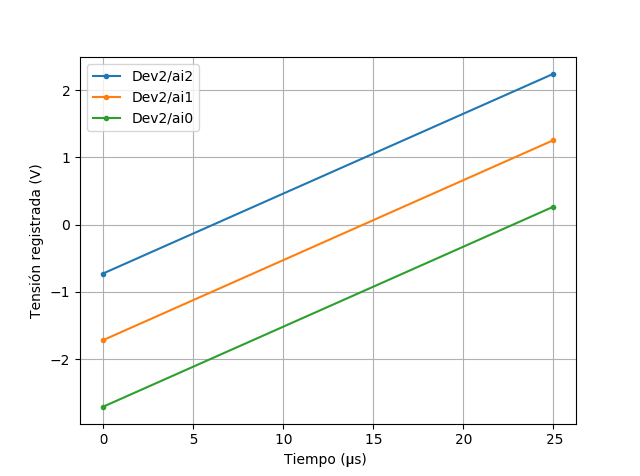
\includegraphics[width=\columnwidth]{figs/multiplex.png}
\label{fig:multiplex}
\caption{Caracterización del multiplexor midiendo una rampa de tensión de manera simultanea en tres canales analógicos.}
\end{figure}


Un resultado típico de este experimento donde se utilizaron tres canales analógicos y una frecuencia de muestreo de 40 kHz se muestra en la figura \ref{fig:multiplex}. En la misma se observan dos eventos de medición separados un período de muestreo. Para cada uno se puede ver que la diferencia entre los valores de tensión registrados en cada canal es la misma y el orden se repite en cada adquisición. A partir de conocer los parámetros de la rampa de tensión utilizada se puede calcular que la diferencia de tensión observada corresponde exactamente a un tercio del período de muestreo. El mismo resultado se obtiene si se utilizan cuatro canales, donde ahora las mediciones se distribuirán equiespaciadamente entre cuatro el período de muestreo. El mismo resultado se observa al cambiar la frecuencia de muestreo. Esto demuestra que la placa de adquisición va digitalizando los canales analógicos de manera secuencial y a intervalos constantes y equiespaciados temporalmente dentro del período de muestreo.

Para finalizar la caracterización de la placa se midió la influencia del \textit{settling time} en las mediciones. Para hacer esto se configuraron dos canales analógicos consecutivos de la placa en las escalas de medición extremas (-200 mV a 200 mV y -10 V a 10 V). Luego se conectó el primero a tierra y el segundo a la referencia de 5 V de la misma placa. A continuación se realizó un barrido de frecuencias de adquisición registrando la tensión detectada en cada canal. El resultado de este experimento se muestra en las figuras \ref{fig:settling1} y \ref{fig:settling2}, donde se graficó la diferencia de tensión medida respecto de la esperada para cada canal. Se observa para los dos casos que a medida que la frecuencia aumenta (y luego se cambia cada vez más rápido de un canal a otro) se obtiene una pequeña señal residual en la dirección de la señal del canal vecino (positiva para el conectado a tierra y negativa para el de 5 V). Esto muestra que la señal está afectada, a frecuencias altas, por el tiempo que tarda la placa en preparar el acondicionamiento de la señal previo a su digitalización.  

\begin{figure}[h!]
\centering
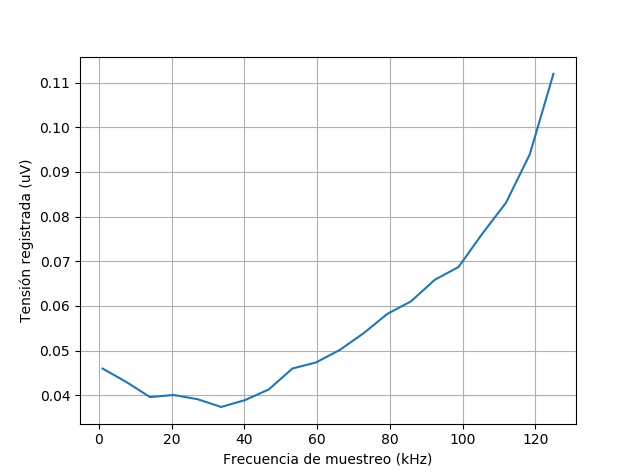
\includegraphics[width=\columnwidth]{figs/settling0V.png}
\label{fig:settling1}
\caption{Señal medida en una entrada conectada a tierra, configurada en $\pm$200 mV contigua a otra configurada en $\pm$10 V en función de la frecuencia de muestreo.}
\end{figure}

\begin{figure}[h!]
\centering
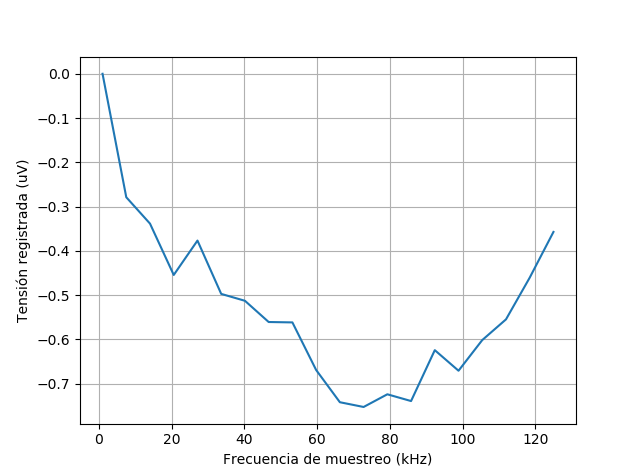
\includegraphics[width=\columnwidth]{figs/settling5V.png}
\label{fig:settling2}
\caption{Variación de la tensión medida en una entrada conectada a 5 V, configurada en $\pm$10 V contigua a otra configurada en $\pm$200 mV en función de la frecuencia de muestreo.}
\end{figure}


\section{Control de temperatura}
\label{sec:control_temperatura}

\subsection{Implementación de un lazo de control}

\subsection{Implementación de un lazo de control PID}




\clearpage

\begin{thebibliography}{99}

	\bibitem{repo} Repositorio en GitHub de la biblioteca propia utilizada en el trabajo, \href{https://github.com/fotonicaOrg/daq}{URL: https://github.com/fotonicaOrg/daq}, actualizado el 7/11/2018. La biblioteca está programada en el archivo \emph{daq.py}.
	\bibitem{nidaqmx} Documentación de la biblioteca nidaqmx, \href{https://nidaqmx-python.readthedocs.io}{URL: https://nidaqmx-python.readthedocs.io}, accedido el 7/11/2018.


\end{thebibliography}



\end{document}
